\chapter{Experiments with Real Aerial Data}
\section{Equipment Setup and Flight Data Collection}
% word checked.
The biggest contribution of the project is that the proposed algorithm
was tested and proven feasible with real flight data collected by the
author. The aerial video and navigation data were collected through a
survey flight with the support of Sander Geophysics Ltd. A main
purpose of the test flight was to obtain aerial video with the camera
close to the ground to mimic the scenario of a low flying UAV. This is
difficult to achieve with any manned fixed wing aircraft since terrain
following flight at low altitude is very dangerous. Therefore, a
helicopter was used to conduct the survey flight to achieve the
terrain following action. To get sensors close to the ground and to
allow for flexible sensor mounting, a simulated unmanned aircraft
system (SUAS) was used to carry all sensors. The SUAS was towed by a
helicopter via a tow rope of 33 meters length (Figure
\ref{fig:towedSUAS}). Yet, sufficient clearance must be established
between the SUAS and the vegetation to prevent the SUAS from being
caught by tree branches. As a result, the helicopter flew a planned
path at approximately 100 meters above ground, and the SUAS was at
approximately 70 meters above ground.

\begin{figure}[h]
\centering
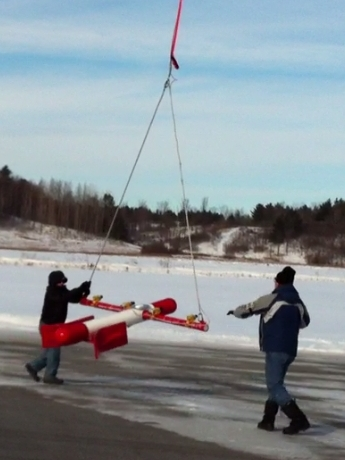
\includegraphics[width=6cm,keepaspectratio=true]{./Figures/SUAS_TAKEOFF2.jpg}
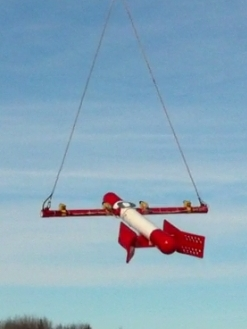
\includegraphics[width=6cm,keepaspectratio=true]{./Figures/SUAS_TAKEOFF3.jpg}
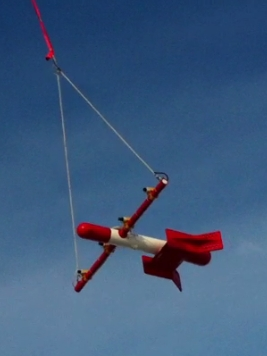
\includegraphics[width=6cm,keepaspectratio=true]{./Figures/SUAS_TAKEOFF4.jpg}
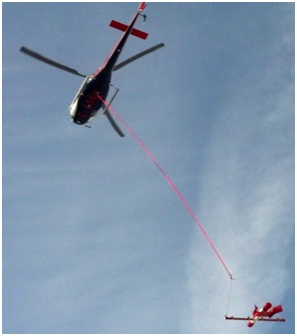
\includegraphics[width=6cm,keepaspectratio=true]{./Figures/towed_SUAS.jpg}
\caption{SUAS towed by a helicopter}
\label{fig:towedSUAS}
\end{figure}
\FloatBarrier

Sensors mounted on the SUAS (Figure \ref{fig:SUAS}) included one wide
angle CCD camera with 6mm focal length lens capturing monocular image
sequences at 30 frames per second, a pair of narrow angle CCD cameras
for binocular image sequences, a GPS antenna, a three-axes fluxgate
sensor, and Athena GS-111m, a flight control INS/GPS navigation unit
\cite{_athena_????} which captures vehicle velocity, acceleration,
rotation, altitude. Analog video and navigation data were sent to the
helicopter via three BNC cables and one data cable for recording.
Installed in the helicopter were two SGL data acquisition systems,
named CDAC. This system records video and navigation data from the
SUAS, as well as data from sensors installed on the helicopter,
including GPS, radar altimeter, laser altimeter, air pressure,
temperature, humidity, etc. (Figure \ref{fig:CDAC}). Videos from the
three cameras were digitized to a resolution of 720 pixels by 480
pixels using three Parvus MPEG4 video encoders installed in the CDACs.
Videos were time-stamped with GPS second on the image screen (Figure
\ref{fig:video_snapshot}) for post-flight synchronization with the
navigation data. Because the test flight recorded data from all
available sensors on board the SUAS and the helicopter, these
recordings would still be useful should any future research require
more sensor data.

\begin{figure}[h]
  \centering
  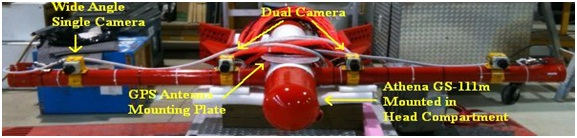
\includegraphics[width=14cm,keepaspectratio=true]{./Figures/SUAS.jpg}
  \caption{Sensors mounting location on SUAS}
  \label{fig:SUAS}
\end{figure}

\begin{figure}[h]
  \centering
  \includegraphics[width=6cm,keepaspectratio=true]{./Figures/athena.jpg}
  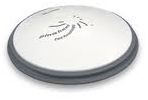
\includegraphics[width=6cm,keepaspectratio=true]{./Figures/GPS_antenna.jpg}
  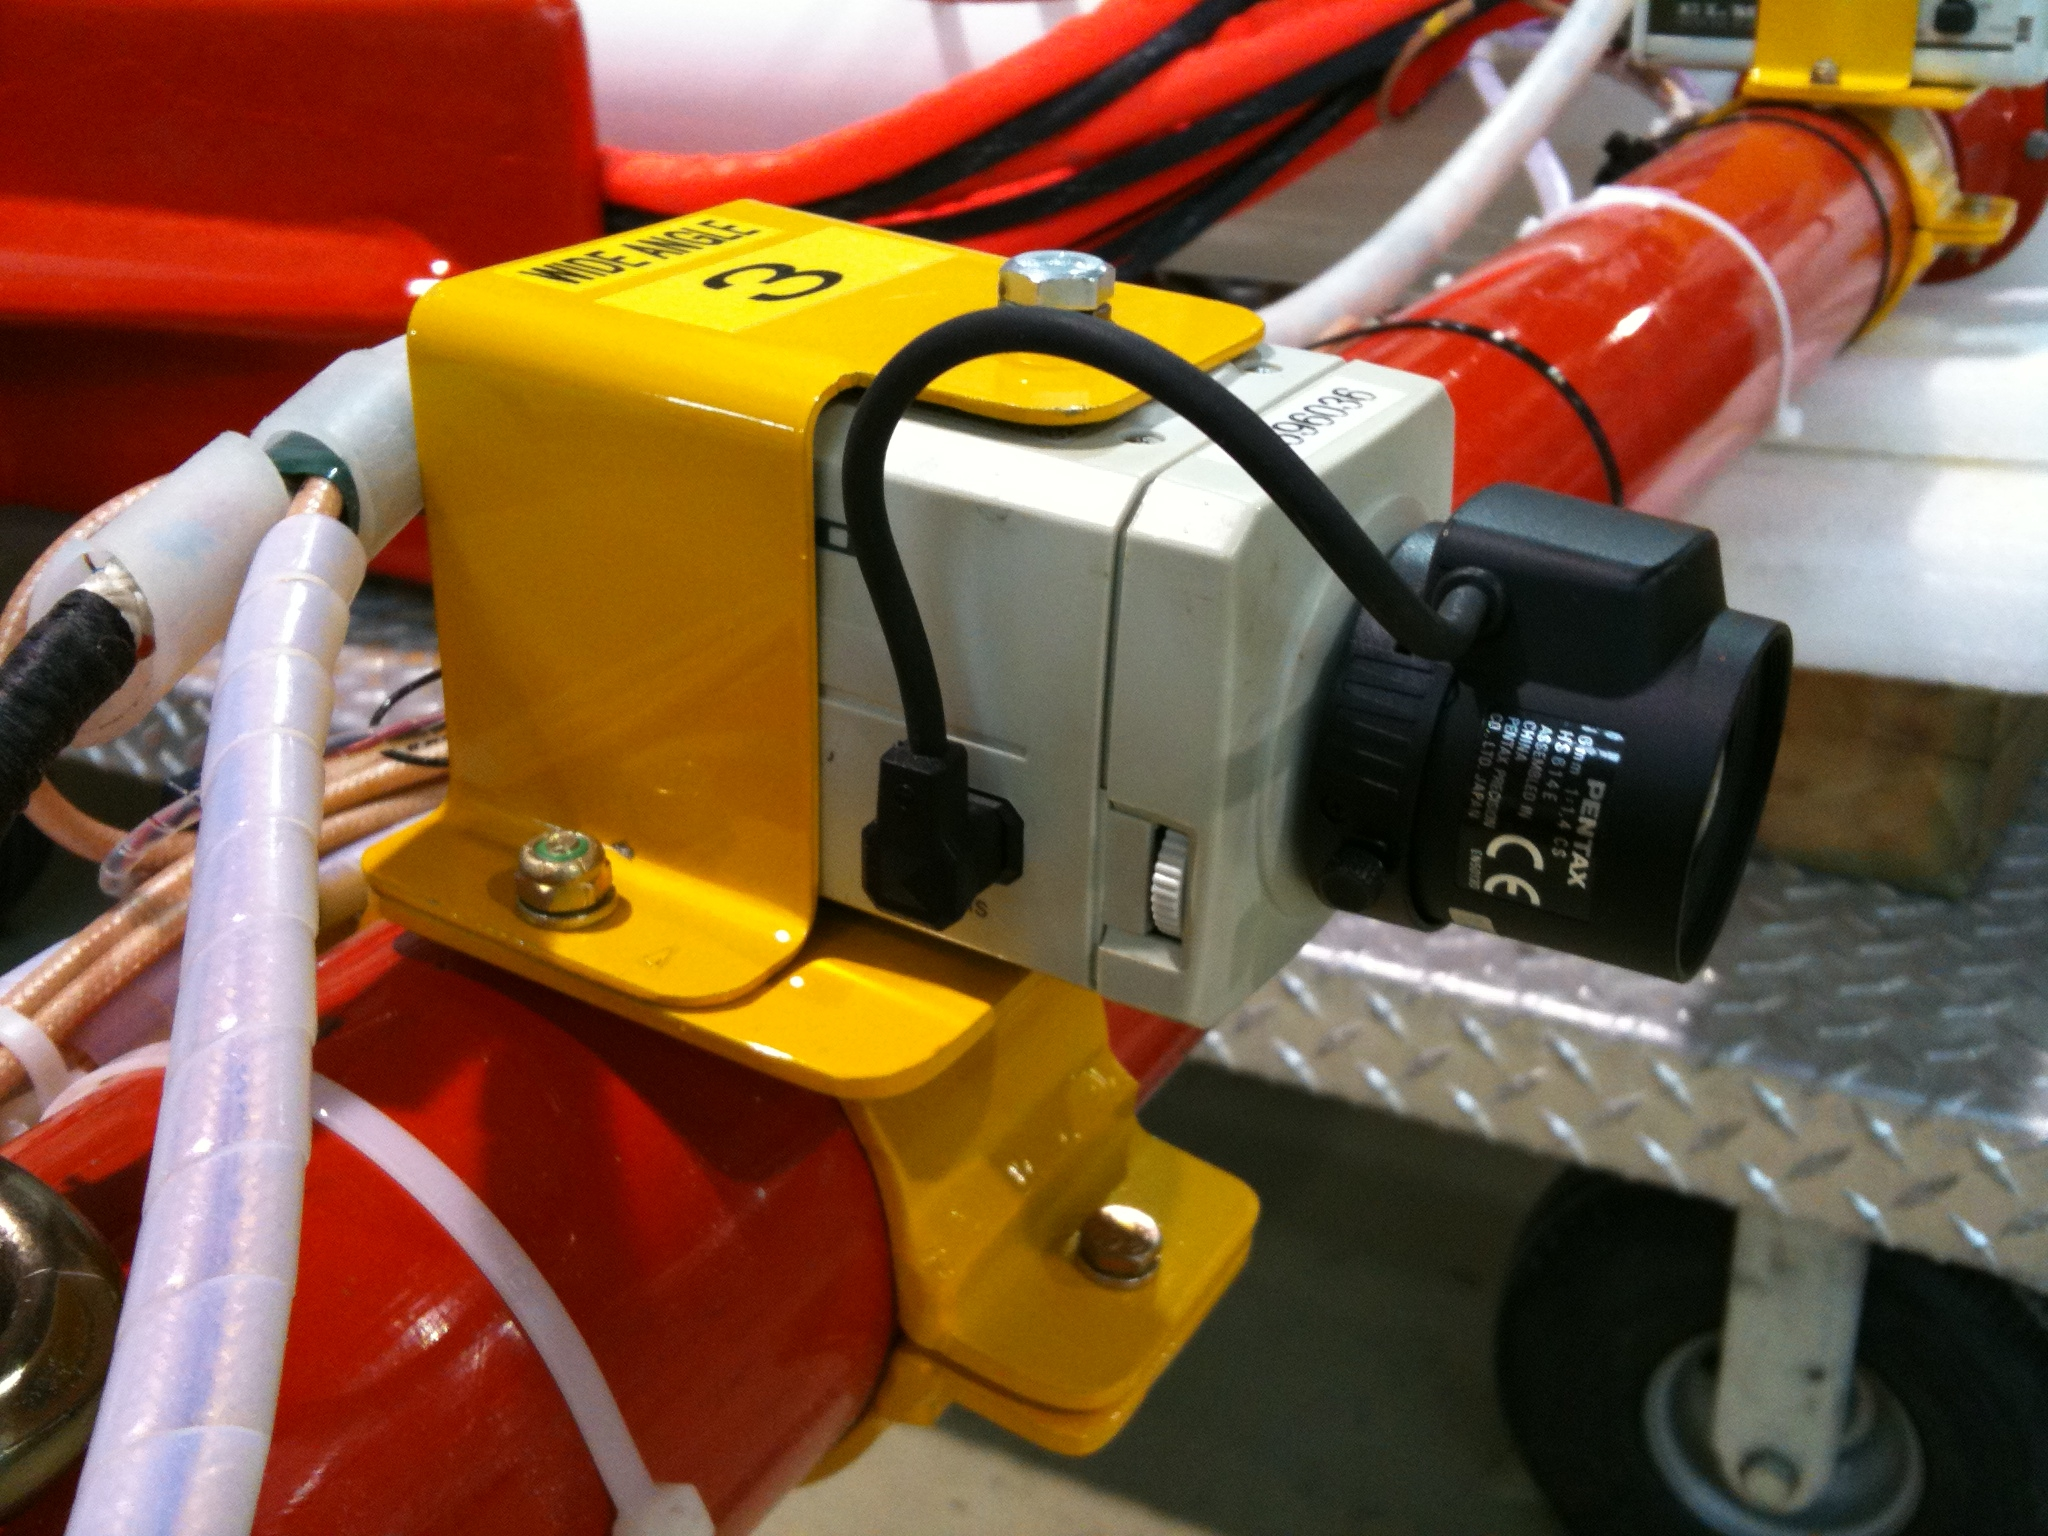
\includegraphics[width=10cm,keepaspectratio=true]{./Figures/wide_cam.jpg}
  \caption{Sensors mounted on SUAS. Top left: Athena
  GS-111m, top right: GPS antenna, bottom: monocular CCD camera}
  \label{fig:SUAS_sensors}
\end{figure}

\begin{figure}[h]
  \centering
  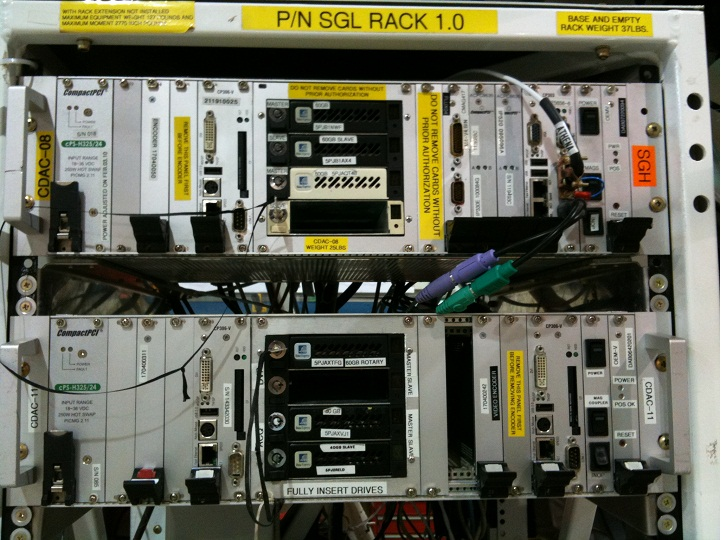
\includegraphics[width=12cm,keepaspectratio=true]{./Figures/CDAC_Rack.jpg}
  \caption{Compact PCI data acquisition system (CDAC)}
  \label{fig:CDAC}
\end{figure}

\begin{figure}[h]
  \centering
  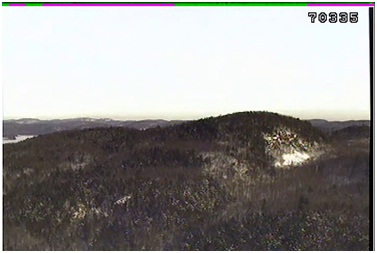
\includegraphics[width=12cm,keepaspectratio=true]{./Figures/video_snapshot.jpg}
  \caption{Image from monocular camera with GPS second timestamp}
  \label{fig:video_snapshot}
\end{figure}

\FloatBarrier

\section{Camera Calibration}\label{sec:camcal}
% word checked
Camera calibration decodes the relation between image pixels and the
actual 3D world. The intrinsic parameters could be affected by a
number of environmental conditions, such as temperature, and humidity.
To extract the camera parameters at a camera condition as close as
possible to the one during test flight, camera calibration was
performed right after the SUAS returned to the SGL hanger. A camera
calibration was done by taking a video of a checkerboard pattern with
various translations and rotations from the camera. A total of 20 views
of the calibration target were chosen from the video, and fed to the
calibration algorithm. A few examples are shown in Figure
\ref{fig:camcal}.

\begin{figure}[h]
  \centering
  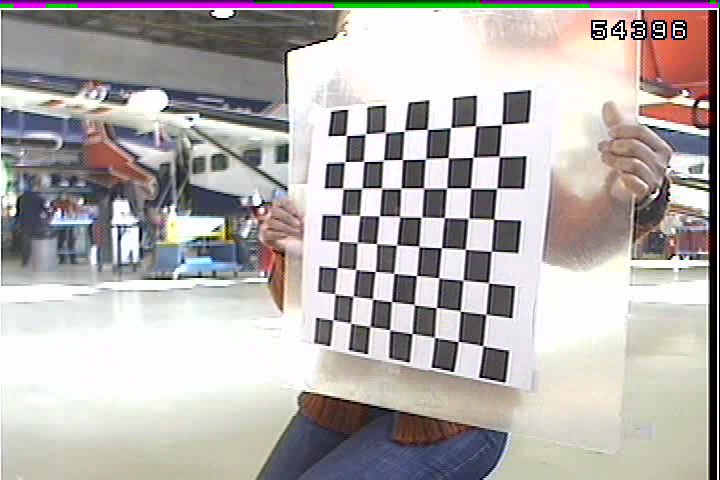
\includegraphics[width=4cm,keepaspectratio=true]{./Figures/camcal/camcal1_130.jpeg}
  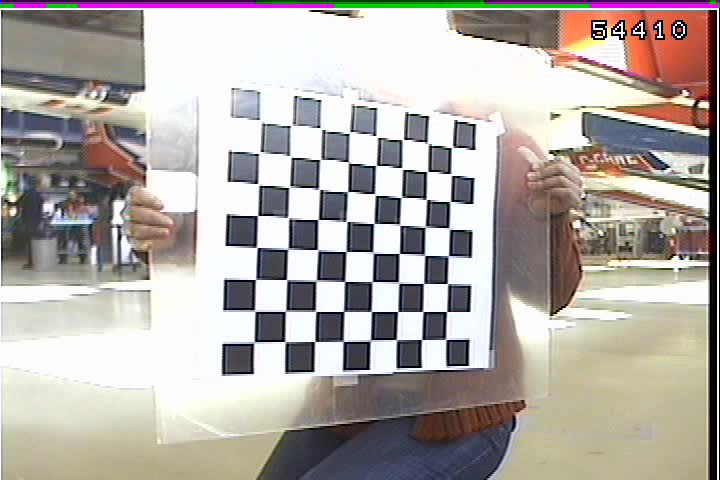
\includegraphics[width=4cm,keepaspectratio=true]{./Figures/camcal/camcal1_140.jpeg}
  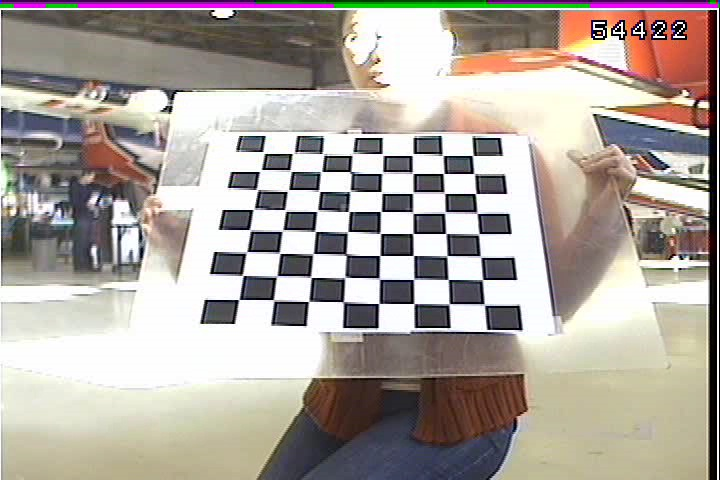
\includegraphics[width=4cm,keepaspectratio=true]{./Figures/camcal/camcal1_160.jpeg}
  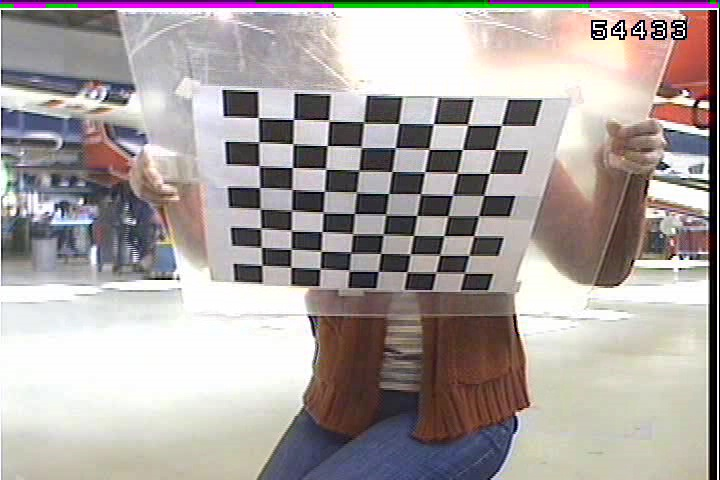
\includegraphics[width=4cm,keepaspectratio=true]{./Figures/camcal/camcal1_180.jpeg}
  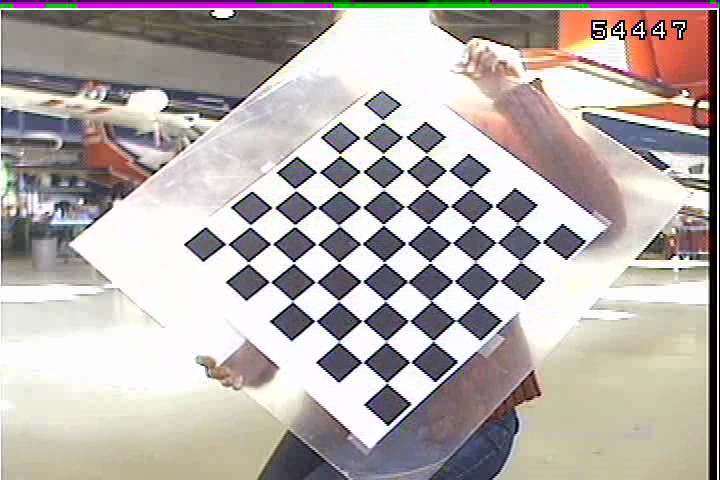
\includegraphics[width=4cm,keepaspectratio=true]{./Figures/camcal/camcal1_210.jpeg}
  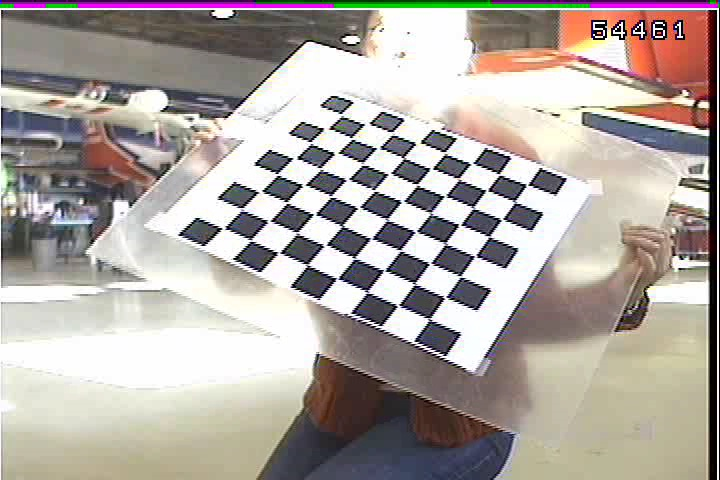
\includegraphics[width=4cm,keepaspectratio=true]{./Figures/camcal/camcal1_240.jpeg}
  \caption{A subset of camera calibration input images}
  \label{fig:camcal}
\end{figure}

The program ``calibration.exe'' was used to calibrate the camera. This
program came with the OpenCV installation. The digitized images have a
resolution of 720 pixels in width and 480 pixels in height. Table
\ref{tab:camcalresult} below lists the calibration results.

\begin{table}[h]
\caption{Camera calibration result}
\label{tab:camcalresult}
\centering
\begin{tabular}{|c|c|}
\hline
Parameter & Result\\ \hline
$f_x$ & 887.6 pixels \\ \hline
$f_y$ & 805.7 pixels\\ \hline
$c_x$ & 381.8 pixels\\ \hline
$c_y$ & 293.7 pixels\\ \hline
$k_1$ & -0.102 \\ \hline
$k_2$ & -0.535 \\ \hline
$p_1$ & 1.15e-003 \\ \hline
$p_2$ & 8.40e-003 \\
\hline
\end{tabular}
\end{table}
\FloatBarrier

\section{Ground Truth Data Collection}
The localization ground truth was obtained through the flight
control unit GS-111m on board the SUAS. The unit recorded the SUAS
position in GPS longitude and latitude coordinates. Orientation was
obtained from the roll pitch and heading measurements. Roll and pitch
accuracy has $0.1^\circ$ and $0.1^\circ$ standard deviation.
Heading accuracy can achieve $0.5^\circ$ \cite{_athena_????}.

Landmark position ground truth came from a digital elevation map (DEM)
downloaded from the CGIAR-CSI website \cite{_cgiar-csi_????}. The DEM
contains longitude, latitude and sea level elevation of the terrain
with a resolution of approximately 100 meters by 100 meters. 

%consider adding the ground truth DEM figure here. 


%%% Local Variables:
%%% mode: latex
%%% TeX-master: "thesis.tex"
%%% End:
